\documentclass[xcolor=pdftex,x11names,table,hyperref]{beamer}

\usepackage{verbatim}
\usepackage{setspace}
\usepackage{url}
\usepackage{xcolor} % See documentation PDF at http://www.ctan.org/pkg/xcolor
\definecolor{darkgreen}{rgb}{0,0.3,0}
\definecolor{darkblue}{rgb}{.05,.05,.30}
\definecolor{lightgrey}{rgb}{0.65,0.65,0.65}
\usepackage{tikzsymbols}


\setbeamertemplate{section in toc}[sections numbered]
\setbeamertemplate{subsection in toc}[subsections numbered]
\setbeamertemplate{subsubsection in toc}[subsubsections numbered]
\usetheme{Singapore}
\setbeamertemplate{navigation symbols}{}
\setbeamertemplate{footline}{%
\vspace{0.0em}%
\hspace{0.5em}%
{\color[rgb]{.1,.1,.1} \insertframenumber{}~/~\inserttotalframenumber}
}

\newcommand{\code}[1]{{\color{darkgreen}\texttt{#1}}}
\newcommand{\detail}[1]{{\color{lightgrey}\small{}#1}}
\newcommand{\teeny}[1]{\scalebox{0.08}{#1}}
\newcommand{\tablecolors}{\rowcolors{2}{blue!12}{white}} % Cool table colors


\begin{document}

\title{Applications of Statistical Language Modeling \\[1.5em]
 %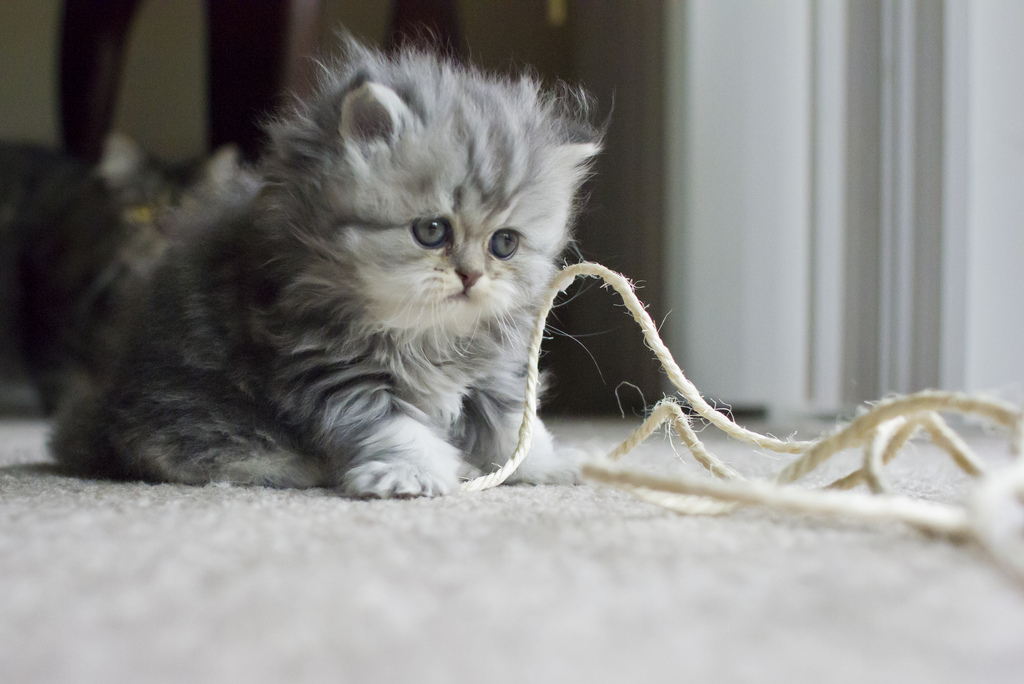
\includegraphics[width=0.5\textwidth]{images/kitten_string_flickr_albaraa.jpg} \\[-1.0em]
 %\small{Possibilities} \\[1.0em]
 %LT1 \\[1.0em]
 }
\author{\href{http://jon.dehdari.org}{Jon Dehdari}}
\frame{\titlepage}

\begin{frame}{Good Morning!}
	\begin{tabular}{ll}
		\parbox[c]{6.5em}{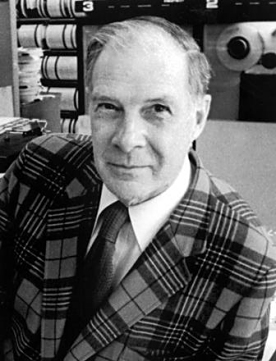
\includegraphics[width=0.28\textheight]{images/Richard_Hamming_from_Wikipedia.jpg} } & \hspace*{1.0em} {\Large Richard Hamming }
	\end{tabular} \\[1.6em]
		``The purpose of computing is insight, not numbers''\\[1.4em]
		\pause
		``If you expect to continue learning all your life, you will be teaching yourself much of the time. You must learn to learn, especially the difficult topic of mathematics.'' \\[1.4em]
		\pause
		``Any unwillingness to learn mathematics today can greatly restrict your possibilities tomorrow.''
\end{frame}


\begin{frame}{Turn That Noise Down!}
	Bayes' Theorem: \\[0.5em]
	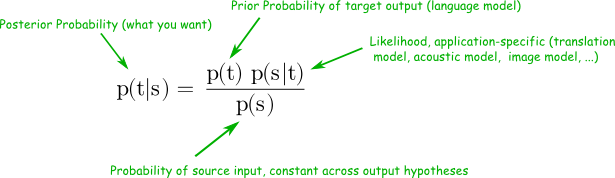
\includegraphics[width=0.90\textwidth]{images/bayes_theorem.png} \\[1.0em]
	\pause
	Noisy Channel Model (applied to translation): \\[0.5em]
	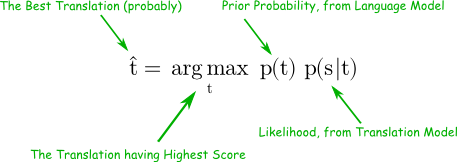
\includegraphics[width=0.86\textwidth]{images/noisy_channel.png}
\end{frame}


\begin{frame}{A Few Uses for Language Models}
 \begin{block}{}
	 Statistical language models ensure fluency in speech recognition (like Siri), machine translation (like Google Translate), on-screen keyboards (smartphones), etc.
 \end{block}
\begin{center}
	
\includegraphics[width=0.14\textwidth]{images/siri.jpg} \hspace{2em}
	
\includegraphics[width=0.15\textwidth]{images/google-translate.jpg} \hspace{2em}
	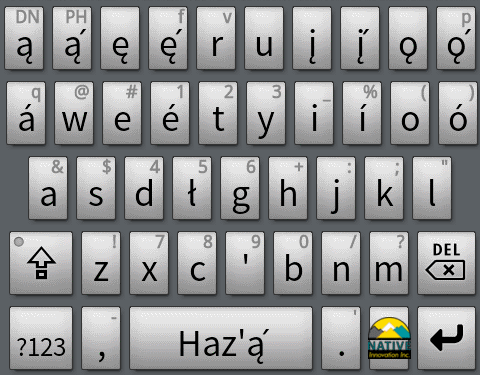
\includegraphics[width=0.15\textwidth]{images/navajo-android-keyboard-crop.png}\\[.1ex]
\end{center}
\end{frame}

\begin{frame}{Actually, There's a Lot of Uses!}
\begin{small}
\begin{spacing}{0.85}
\begin{itemize}
 \item Google suggest
 \item Machine translation
 \item Assisting people with motor disabilities.  For example, \href{https://en.wikipedia.org/wiki/Dasher_(software)}{Dasher}
 \item Speech Recognition (ASR)
 \item Optical character recognition (OCR) and handwriting recognition
 \item Information retrieval / search engines
 \item Data compression
 \item Language identification, as well as genre, dialect, and idiolect identification (authorship identification)
 \item Software keyboards
 \item Surface realization in natural language generation
 \item Image caption generation
 \item Email response generation
 \item Password cracking
 \item Cipher cracking
\end{itemize}
\end{spacing}
\end{small}
\end{frame}

\begin{frame}{Differences in LM Uses}
%\begin{footnotesize}
\scalebox{0.84}{%
\hspace*{-1.7em}%
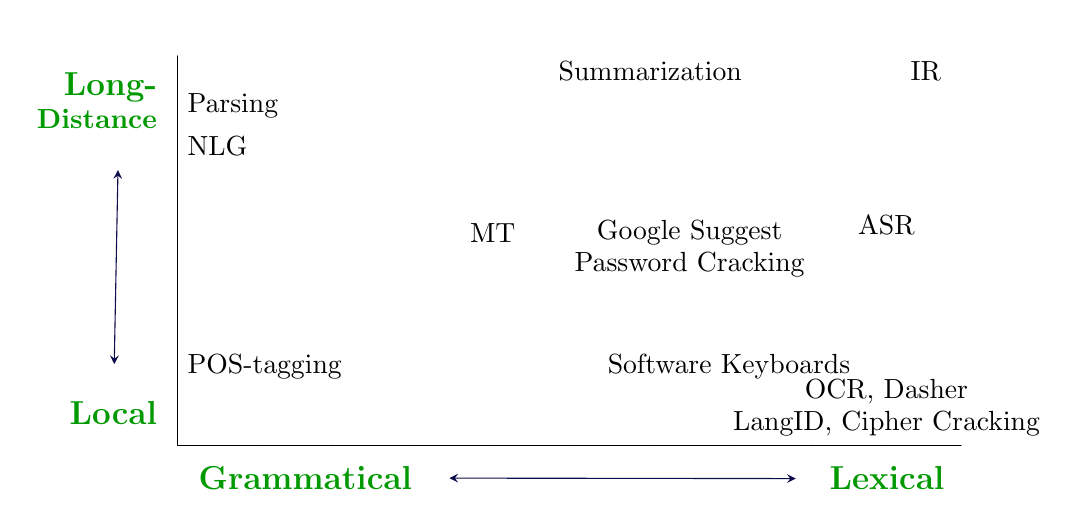
\begin{tikzpicture}[->,>=stealth,line cap=round,shorten >=10pt, shorten <=10pt]
	\node (grammatical) [green!60!black,below right=4pt] at (0,0)  {\large\textbf{Grammatical}};
	\node (lexical) [green!60!black,below left=4pt]  at (10,0) {\large\textbf{Lexical}};
	\draw[-] (-0.35,0) to (10.3,0);
	\draw[<->,darkblue] (grammatical) to (8.2,-0.42);
	\node (local) [green!60!black,above left=4pt, align=right] at (0,0)  {\large\textbf{Local}};
	\node (longdist) [green!60!black,below left=4pt, align=right] at (0,5)  {\large\textbf{Long-}\\\textbf{Distance}};
	%\draw[<->,darkblue] (local) to (longdist);
	\draw[<->,darkblue] (local) to (-0.753,3.85);
	\draw[-] (0,-0.35) to (0,5.3);

	\draw[line width=0.0001pt, white] (0,0) grid (10,5);

	\node [below right] at (0,4.6) {Parsing};
	\node [below] at (6,5) {Summarization};
	\node [below] at (9.5,5) {IR};
	\node [right] at (0,3.8) {NLG};
	\node [right] at (0,1.0) {POS-tagging};
	\node [] at (4,2.7) {MT};
	\node [] at (6.5,2.7) {Google Suggest};
	\node [] at (6.5,2.3) {Password Cracking};
	\node [] at (9,2.8) {ASR};
	%\node [] at (,) {Dasher};
	\node [] at (7,1) {Software Keyboards};
	\node [above] at (9,0.4) {OCR, Dasher};
	\node [above] at (9,0) {LangID, Cipher Cracking};
\end{tikzpicture}
}\\
\vspace*{3.0em}
\teeny{Actually parsers and POS-taggers aren't applications of language models, but rather they are types of language models.}
\end{frame}

\begin{frame}{LM Usage}
\begin{block}{Typical LM Queries in ...}
	\begin{small}
	\begin{description}
	\item[ASR]: p(recognize speech) vs.\ p(wreck a nice beach) vs.\ p(wreck an ice peach), ...
	\item[Cipher cracking]: p(attack at dawn) vs.\ p(uebvmkdvkdbsqk)
	\item[Google Suggest]: p(how to cook french fries) vs.\ p(how to cook french dictionary)
	\item[MT \& NLG]: lex: p(use the force) vs.\ p(use the power); \\ ordering: p(ready are you) vs.\ p(are you ready)
	\item[OCR]: p(today is your day) vs.\ p(+qdav ls y0ur d4ij)
	\item[IR]: query(cats and the cradle): doc1(i like cats) vs.\ doc2(i like dogs)
	\item[LangID]: query(a blue watch): lang1(the green witch \ldots) vs.\ lang2(la bruja verde \ldots)
	\end{description}
	\end{small}
\end{block}
\teeny{A good cipher should obey the principle of diffusion (\href{http://netlab.cs.ucla.edu/wiki/files/shannon1949.pdf}{Shannon, 1949}).}
\end{frame}


\begin{frame}{Language Modeling is Interesting!}
 \begin{block}{}

\begin{center}
\begin{small}
\begin{spacing}{1.4}
\tablecolors
\begin{tabular}{l|l}
	\hline
	\bf NLP Task & \bf Avg.\ Entropy \\
	\hline
	\hline
	Language Modeling (=Word Prediction) & 7.12 \\
	English-Chinese Translation & 5.17 \\
	English-French Translation & 3.92 \\
	QA (Open Domain) & 3.87 \\
	Syntactic Parsing & 1.18 \\
	QA (Multi-class Classification) & 1.08 \\
	Text Classification (20 News) & 0.70 \\
	Sentiment Analysis & 0.58 \\
	Part-of-Speech Tagging & 0.42 \\
	Named Entity Recognition & 0.31 \\
	\hline
\end{tabular}
\end{spacing}
\end{small}
\end{center}
\vspace*{-2.3em}
\end{block}
\vspace*{-0.5em}
\tiny{From Li \& Hovy (2015)\nocite{li-hovy2015}}
\end{frame}

\begin{frame}{Illustration with Image Caption Generation}
	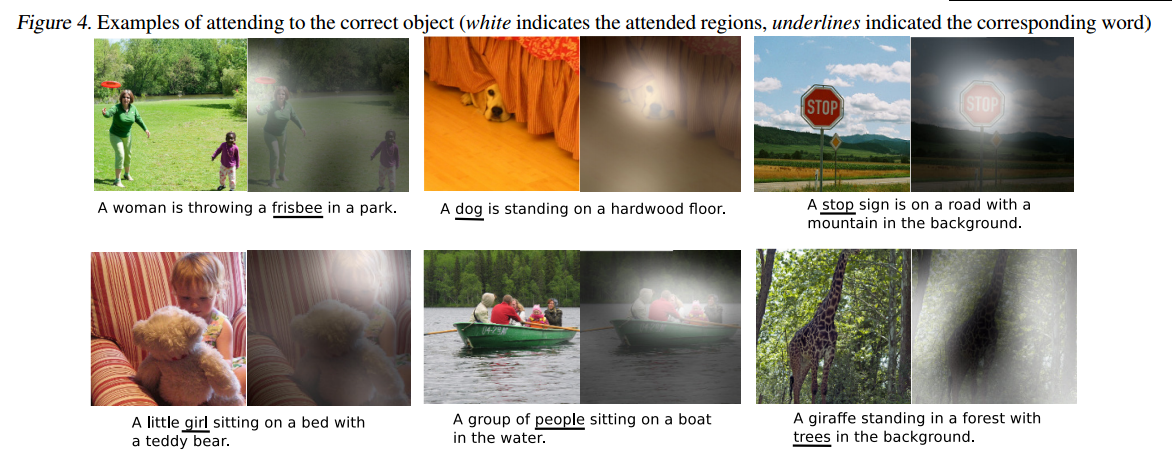
\includegraphics[width=1.03\textwidth]{images/xu-etal2015_icml_fig4.png} \\[1.5em]
	\tiny{From Xu et al (2015; ICML, Fig.\,4)\nocite{xu-etal2015}}.  This uses the neural attention model, which we'll discuss later in the semester.
\end{frame}





% \begin{frame}{}
% \begin{itemize}
% 	\item 
% 	\item 
% 	\item 
% \end{itemize}
% \end{frame}


\end{document}
